\documentclass[twoside,twocolumn]{article}

\usepackage{blindtext} 
\usepackage{graphicx}
\usepackage[sc]{mathpazo} 
\usepackage[T1]{fontenc} 
\linespread{1.05} 
\usepackage{microtype} 

\usepackage[utf8]{inputenc} 


\usepackage[spanish,english]{babel} 



\usepackage[hmarginratio=1:1,top=32mm,columnsep=20pt]{geometry} 
\usepackage[hang, small,labelfont=bf,up,textfont=it,up]{caption} 
\usepackage{booktabs} 


\usepackage{lettrine} 


\usepackage{enumitem} 
\setlist[itemize]{noitemsep} 


\usepackage{abstract} 
\renewcommand{\abstractnamefont}{\normalfont\bfseries} 
\renewcommand{\abstracttextfont}{\normalfont\small\itshape} 


\usepackage{titlesec} 
\renewcommand\thesection{\Roman{section}} % 
\renewcommand\thesubsection{\roman{subsection}} 
\titleformat{\section}[block]{\large\scshape\centering}{\thesection.}{1em}{} 
\titleformat{\subsection}[block]{\large}{\thesubsection.}{1em}{} 


\usepackage{fancyhdr} 
\pagestyle{fancy} 
\fancyhead{} 
\fancyfoot{} 
\fancyhead[C]{Patrones de Diseño $\bullet$ Octubre 2020 $\bullet$ } 
\fancyfoot[RO,LE]{\thepage} 


\usepackage{titling} 


\usepackage{hyperref} 

\usepackage{listings}
\usepackage{xcolor}

\lstdefinestyle{sharpc}{language=[Sharp]C, frame=lr, rulecolor=\color{blue!80!black}}


%----------------------------------------------------------------------------------------
%	TILULOS
%----------------------------------------------------------------------------------------


\setlength{\droptitle}{-4\baselineskip} 

\pretitle{\begin{center}\Huge\bfseries} 
\posttitle{\end{center}} 
\title{Patrones de Diseño} 
\author{Percy Taquila Carazas, Katerin Merino Quispe, Abraham Lipa Calabilla,
\\Edwart Balcon Coahila, Lisbeth Espinoza Caso}
\date{\today} 
\renewcommand{\maketitlehookd}{

\selectlanguage{english}
\begin{abstract}
\noindent 

\end{abstract}


\selectlanguage{spanish}
\begin{abstract}
\noindent 
Los patrones de diseño dan un mecanismo codificado para describir problemas y su solución en forma tal que permiten que la comunidad de ingeniería de software diseñe el conocimiento para que sea reutilizado.
Un patrón describe un problema, indica el contexto y permite que el usuario entienda el ambiente en el que sucede el problema, y enlista un sistema de fuerzas que indican cómo puede interpretarse el problema en su contexto, y el modo en el que se aplica la solución.
El patron Abstract Factory suele implementarse con metodos de fabricacion que tambien generalmente son llamados desde el interior de Template Method.
\end{abstract}

}

%----------------------------------------------------------------------------------------

\begin{document}

% Print the title
\maketitle

%----------------------------------------------------------------------------------------
%	INTRODUCCION
%----------------------------------------------------------------------------------------

\section{Introduccion}

\lettrine[nindent=0em,lines=3]{L}os



%----------------------------------------------------------------------------------------
%	Desarrollo
%----------------------------------------------------------------------------------------


\section{Desarrollo}




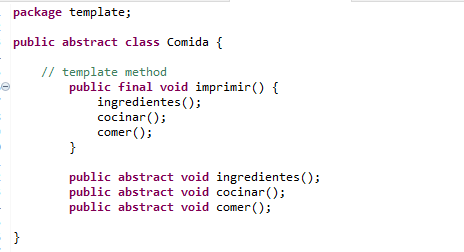
\includegraphics[width=8cm]{Imagenes/imagen}

La clase Hamburguesa extiende de Comida e implementa los tres métodos abstractos de Comida.



%----------------------------------------------------------------------------------------
%	Conclusiones
%----------------------------------------------------------------------------------------


\section{Conclusiones}

La conclusión 
%----------------------------------------------------------------------------------------
%	Recomendaciones
%----------------------------------------------------------------------------------------

\section{Recomendaciones}


\begin{itemize}
\item Cuando se conoce el efecto colateral que conlleva el patrón de diseño y es viable la aparición de este efecto.
\item Suministrar alternativas de diseño para poder tener un software flexible y reutilizable.

\end{itemize}



%----------------------------------------------------------------------------------------
%	BIBLIOGRAFIA
%----------------------------------------------------------------------------------------

\selectlanguage{spanish}
\begin{thebibliography}{99} 

\bibitem[1]{}
\newblock Gamma, Erich; Helm, Richard; Johnson, Ralph; Vlissides, John(1995).Design Patterns: Elements of Reusable Object- Oriented Software. Reading,Massachusetts: Addison Wesley Longman, Inc.

\bibitem[2]{}
\newblock Nesteruk, D. (2019). Design Patterns in .NET: Reusable Approaches C\# in and F\# for Object-Oriented Software Design (1st ed.). Apress.

\bibitem[3]{}
\newblock Patrones de Diseño. Elementos de software orientado a objetos reutilizable. ERICH GAMMA. RICHARD HELM. RALPH JOHNSON. JOHN VLISSIDES.

\bibitem[4]{}
\newblock Patrones de diseño en Java: Los 23 modelos de diseño: descripción y solución ilustradas en UML 2 y Java Autor: Laurent Debrauwer

\end{thebibliography}


%----------------------------------------------------------------------------------------


\end{document}
